Même si on ne l'a pas vu dans le cours sur la programation impérative et que ce n'est pas le but de l'exercice, comme le projet s'y prête beaucoup, on a décidé d'avoir une approche orientée objet.
Cela n'était pas possible en ada, mais depuis 1995 (Ada95), le langage a été adapté pour la POO (Programmation Orientiée Objet). On a donc créé une classe mère \lstinline{Google}, et deux classes filles \lstinline{Google_Naive} et \lstinline{Google_Creuse}. La classe mère définit toutes les fonctions et procédures, sans qu'elles ne soient implémentées (leur corps n'est composé que de la ligne \lstinline{null;}).
Les classes filles \textit{override} ces fonctions et procédures.
\begin{figure}[ht!]
   \centering
   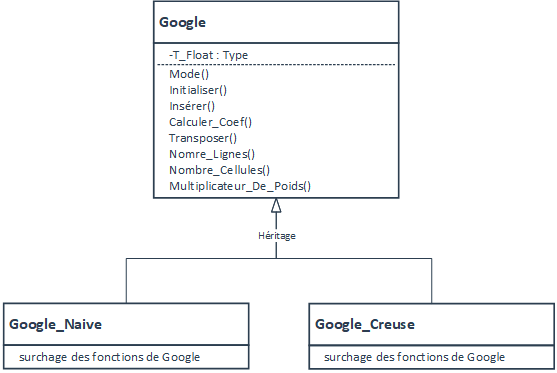
\includegraphics[scale=0.5]{partie-2/sous-partie-3/heritage.png}
   \caption{Héritage de la classe Google \label{fig : heritage_projet}}
\end{figure} 
En Ada voici comment se code un \textit{objet} :

\begin{lstlisting}[caption={POO en Ada - Définition}, label={poo-ada-def}]
   type Classe_Mere is tagged null record;

   procedure Procedure_1 (Self : in out Classe_Mere);
   procedure Procedure_2 (Self : in out Classe_Mere; Un_Argument : in Integer);

   type Classe_Fille is new Classe_Mere with record
      Parametre : Float;
   end record;

   procedure Procedure_2 (Self : in out Classe_Fille);
\end{lstlisting}

Avec son implémentation :

\begin{lstlisting}[caption={POO en Ada - Implémentation}, label={poo-ada-imp}]   
   procedure Procedure_1 (Self : in out Classe_Mere) is
   begin
      null;
   end Procedure_1;
   procedure Procedure_2 (Self : in out Classe_Mere; Un_Argument : in Integer)

   begin
      null;
   end Procedure_2;
   procedure Procedure_2 (Self : in out Classe_Fille; Un_Argument : in Float)

   begin
      null;
   end Procedure_2;

   ...

   declare
      A : Classe_Mere;
      B : Classe_Fille;
   begin
      A.Procedure_1;
      A.Procedure_2(4);

      B.Procedure_1;
      B.Procedure_2(0.59);
   end;
\end{lstlisting}